\documentclass[10pt]{article}

\usepackage[utf8x]{inputenc}
\usepackage[T1]{fontenc}
\usepackage[finnish]{babel}
\usepackage{amsmath}
\usepackage{amssymb}
\usepackage{amsfonts}
\usepackage{amsthm}
\usepackage{graphicx}
\usepackage[ruled]{algorithm2e}
\usepackage{empheq}
\usepackage{float}
\usepackage{graphicx}
\usepackage{color}
\usepackage{hyperref}
\usepackage{tocloft}
\usepackage{fancyvrb}
\renewcommand{\cftsecleader}{\cftdotfill{\cftdotsep}}

\makeatletter
\g@addto@macro\cftsecfont{\bfseries}
\g@addto@macro\cftsubsecfont{\bfseries}

\g@addto@macro\cftsecpagefont{\bfseries}
\g@addto@macro\cftsubsecpagefont{\bfseries}

\title{Tietokantasovellus -- Dokumentaatio}
\date{2014, periodi 4}
\author{Rodion ``rodde'' Efremov}
\renewcommand*\rmdefault{iwona}
\definecolor{logobg}{RGB}{31,124,255}

\begin{document}

\pagenumbering{Roman}
\centerline{\colorbox{white}{\begin{minipage}{12cm}
\maketitle
\end{minipage}}}
\pagecolor{logobg}

\begin{center}
\centerline{
\includegraphics[width=450px, height=200px]{multilogo}}
\end{center}

\newpage
\pagecolor{white}
\tableofcontents
\newpage
\pagenumbering{arabic}

\section{Johdanto} Tämä dokumentti on tarkoitettu kuvaamaan Tietokantasovellus-kurssin (582203) aikana toteutettu verkkosovellus. Ajallisesti ottaen kurssisuoritukseni on ajoitettu kevään 2014 neljännelle periodille. Harjoitustyön aiheena on \href{http://advancedkittenry.github.io/suunnittelu_ja_tyoymparisto/aiheet/Keskustelufoorumi.html}{Keskustelufoorumi} ja järjestelmän nimi on \textbf{multilog}. multilog ei paljon eroa phpBB:stä, mutta todennäköisesti tulee olemaan yksinkertaisempi ainakin sivujen tyylityksen osalta. Kuten yleensäkin, multilog:n on tarkoitus olla helppokäyttöinen ja ilmainen palvelu, jossa käyttäjäkunta pääsee keskustelemaan vapaasti. Toteutuskieleksi olen valinnut Javan (servletit Tomcat:n ajettavaksi), ja tietokannaksi olen valinnut niin ikään suositeltu PostgreSQL. Tarkkaanottaen, toteutus perustuu Java EE 5 spesifikaation, joten ohjelmisto voi ajaa ainakin Tomcat 6:ssa.
Saadakseen postausten tyylittely toimimaan, käyttäjän selaimen on tuettava Javascript. Sovelluksen liittyvät SQL-toiminnot todennäköisesti ei saada standardinmukaisiksi, jotenka järjestelmä on sidottu PostgreSQL:n käyttöön tietokantanaan.

\section{Yleiskuva järjestelmästä (multilog)}
Aiheenani on keskustelufoorumin toteuttaminen. Järjestelmässä on kolme käyttäjäkategoriaa: 
\begin{itemize}
  \item ylläpitäjä (admin),
  \item moderaattori (moderator),
  \item käyttäjä (user).
\end{itemize}
Käyttäjä voi luoda tunnuksensa rekisteröitymällä sovellukseen. Ensimmäinen ylläpitäjä on luotu SQL-komennosta. Myöhemmin kun järjestelmässä alkaa olla käyttäjiä, ylläpitäjä voi ylentää tavallisen käyttäjän moderaattoriksi tai suoraan ylläpitäjäksi. Ylläpitäjä voi pudottaa moderaattorin peruskäyttäjäksi ja poistaa mielivaltaisen käyttäjän, jolloin myös moderaattoreiden poisto on mahdollista. Lisäksi, mikä tahansa rekisteröitynyt henkilö voi poistaa profiilinsa. Mitä tulee tilanteeseen, jossa ylläpitäjä poistaa itseään, onnistuu se vain jos poiston jälkeen järjestelmään jää vähintään yksi muu ylläpitäjä. (Järjestelmässä pitää olla vähintään yksi ylläpitäjä.) Moderaattori voi poistaa käyttäjien viestit, mikäli siihen on tarvetta. Lisäksi, moderaattori voi asettaa käyttäjät maksimissaan 7 vuorokauden käyttökieltoon. Toisaalta, moderaattori voi ylentää käyttäjän moderaattoriksi. Mitä tulee keskustelusäikeisiin, uusien luonti onnistuu jo peruskäyttäjän oikeuksilla; säikeiden poistaaminen vaatii vähintään moderaattorin oikeudet. Ylläpitäjät pystyvät tekemään samat toiminnot kuin moderaattoritkin. 

Mitä tulee itse foorumin rakenteeseen, alkusivulla voi selata ``teemoja''. Jokainen teema pitää sisällään vähintään yhden ``säikeen'', joista jälkimmäinen pitää sisällään siihen liittyvän keskusteluhistorian. Teemojen luonti ja poistaminen vaatii ylläpitäjän. Keskustelun lisäksi jokainen käyttäjä/moderaattori/ylläpitäjä voi lähettää yksityiset viestit mielivaltaiselle käyttäjälle ilman statusrajoja. Sovellus luo jokaiselle käyttäjälle profiilisivun, joissa näytetään (profiilin omistajan halutessa) sähköpostiosoite, syntymäpäivä, sukupuoli, oikea nimi. Profiilisivuilla esitetään aina (edes oletus-) avatar-kuva, lista postauksia ja postausten määrä.

Rekisteöityessään käyttäjä voi halutessaan lisätä avatar-kuvan, joka skaalataan tietynkokoiseksi; muussa tapauksessa käytetään oletus-avatar. Avatarkuvan voi lisätä/poistaa ja tiedot päivittää myös rekisteröitymisen jälkeen.

multilog sallii viesteissä erityistagien kirjoittamisen, joilla tekstiä pystyy muotoilemaan; alustavasti seuraavat muotoilut toteutetaan:
\begin{itemize}
  \item kursivointi,
  \item lihavointi,
  \item kiinteävälinen tekstitys (monospaced font),
  \item linkkien upottaminen,
  \item kuvien linkkittäminen tekstiin.
\end{itemize}

\subsection{Käyttötapaukset}
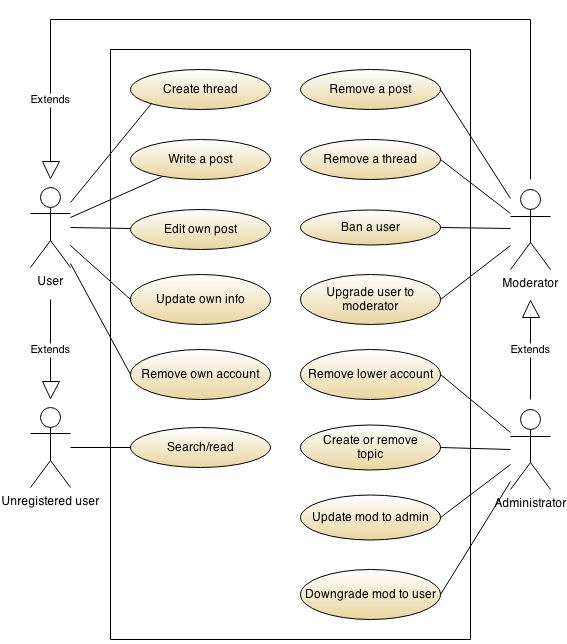
\includegraphics[width=\textwidth, height=0.9\textheight, keepaspectratio]{multilogUseCaseDiagram}

\noindent Huomaa, että kaikki toiminnot paitsi lukeminen ja haku edellyttävät sisäänkirjautumisen.
\subsection{Käyttäjäryhmät}
\begin{description}
  \item[Jokamies] \hfill \\
  Henkilö joka ei ole rekisteröitynyt \textbf{multilog}:iin. Voi hakea ja lukea järjestelmässä olevat postaukset.
  \item[Peruskäyttäjä (user)] \hfill \\
  Rekisteröitynyt peruskäyttäjä, joka voi luoda säikeet ja postaukset, vastata olemassaoleviin postauksiin, muokata tietojaan ja poistaa profiilinsa. Perii myös \textbf{jokamiehen} toiminnot.
  \item[Moderaattori (moderator)] \hfill \\
  Käyttäjä, joka voi poistaa säikeet ja postaukset, ylentää \textbf{peruskäyttäjän} moderaattoriksi ja aseta peruskäyttäjät käyttökieltoon. Perii myös \textbf{peruskäyttäjän} toiminnot.
  \item[Ylläpitäjä (admin)] \hfill \\
  Ylläpitäjä, joka voi ylentää peruskäyttäjän/moderaattorin ylläpitäjäksi, poistaa ei-ylläpitäjäkäyttäjän, luoda/poistaa aiheet. Perii myös \textbf{moderaattorin} toiminnot.
\end{description}

\subsection{Käyttötapauskuvaukset}
\begin{Verbatim}[frame=single]
Jokamiehen käyttötapaukset
    Haku:  
      Postausten, säikeiden, teemojen ja profiilien haku
    Lukeminen:
      Haetun sisällön lukeminen
\end{Verbatim}

\begin{Verbatim}[frame=single]
Peruskäyttäjän käyttötapaukset
  Säikeen luonti:
    Peruskäyttäjä voi luoda säikeen teeman alle
  Kirjoittaminen:
    Peruskäyttäjä voi kirjoittaa säikeessä
  Vastaaminen:
    Peruskäyttäjä voi vastata olemassa olevaan viestiin
  Muokkaaminen:
    Peruskäyttäjä voi muokata omat viestit
  Tietojen päivittäminen:
    Peruskäyttäjä voi päivittää henkilötietojaan; 
    myös poistaamaan tilinsä
    
 ** Peruskäyttäjä perii kaikki jokamiehen toiminnot **
\end{Verbatim}

\newpage

\begin{Verbatim}[frame=single]
Moderaattorin käyttötapaukset
  Säikeen poisto:
    Moderaattori voi poistaa mielivaltaisen säikeen
  Käyttökiellon asettaminen:
    Moderaattori voi aseta mielivaltaisen peruskäyttäjän 
    käyttökieltoon (maksimissaan 7 päiväksi)
  Putsaaminen:
    Moderaattori voi poistaa mielivaltaisen peruskäyttäjän viestin
  Ylentäminen:
    Moderaattori voi promotoida peruskäyttäjän moderaattoriksi
    
** Moderattori perii kaikki peruskäyttään toiminnot  **
\end{Verbatim}

\begin{Verbatim}[frame=single]
Ylläpitäjän käyttötapaukset
  Y.1 Ylentäminen:
    Ylläpitäjä voi promotoida moderaattorin ylläpitäjäksi
  Y.2 Alentaminen:
    Ylläpitäjä void alentaa moderaattorin peruskäyttäjäksi
  Y.3 Käyttäjän poisto:
    Ylläpitäjä voi poistaa peruskäyttäjän
    (Y.2:n nojalla myös moderaattorin)
    
** Ylläpitäjä perii kaikki moderaattorin toiminnot **
\end{Verbatim}

\section{Käyttöliittymä}
Sovelluksen pääsivulla tulee olemaan 4 linkkiä:
\begin{description}
  \item[Search] sovelluksen hakutoiminto,
  \item[Browse] ohjaa teemat sisältävälle sivulle, josta pääsee katsomaan kunkin teeman säikeet, joissa, puolestaan, pääsee lukemaan postaukset,
  \item[Sign in] ohjaa sisäänkirjautumissivulle,
  \item[Sign up] ohjaa rekisteröimissivulle.
\end{description}
\textbf{Search} - linkin takana on sivu, jossa käyttäjä voi kirjoittaa epätriviaaleja hakulausekkeita, joissa on operaattorit \textbf{NOT}, \textbf{AND} ja \textbf{OR}, joiden lisäksi on valitsimet \textit{post}, \textit{author}, \textit{topic} ja \textit{thread}. \textbf{Browse} - linkin takana on puolestaan lista teemoja, joita klikkaamalla pääsee listaan säikeitä, joita klikkaamalla pääsee lukemaan ko. säikeen postaukset (käyttäjän ollessa kirjautunut pääsee kirjoittamaan oman postauksen tai vastaamaan olemassaolevaan postaukseen). \textbf{Sign up} - linkin takana on sivu, jossa voi luoda peruskäyttäjän profiiliin ja \textbf{Sign in} - linkin takana järjestelmään voi kirjautua.

Käyttäjän ollessa kirjautunut, navigointipalkin oikealla puolella on linkit \- \textbf{Account} ja \textbf{Sign out}, joilla voi mennä oman tilin hallintasivulle tai kirjautua ulos vastaavasti. Jokainen \textit{kirjautunut} käyttäjä $K_1$ voi lukea toisen käyttäjän $K_2$ tiedot sivulla $S$: lukjan $K_1$ ollessa korkeamalla käyttäjätasolla, voi hän promotoida $K_2$:n enintään $K_1$:n tasolle painamalla painiketta sivulla $S$.

Kirjautuneen käyttäjän selatessa säikeen viestit, voi hän painaa postauksen yhteydessä olevaa \textbf{Reply} - painiketta ja vastata siihen. Ellei käyttäjä halua nimenomaan vastata mihinkään postaukseen, voi hän kirjoittaa säikeen lopussa olevaan postauslaatikkoon, jolloin luodaan viesti vailla ``vanhempiviestiä''.
\begin{figure}
  \caption{Päänäkymä}
  \centering
  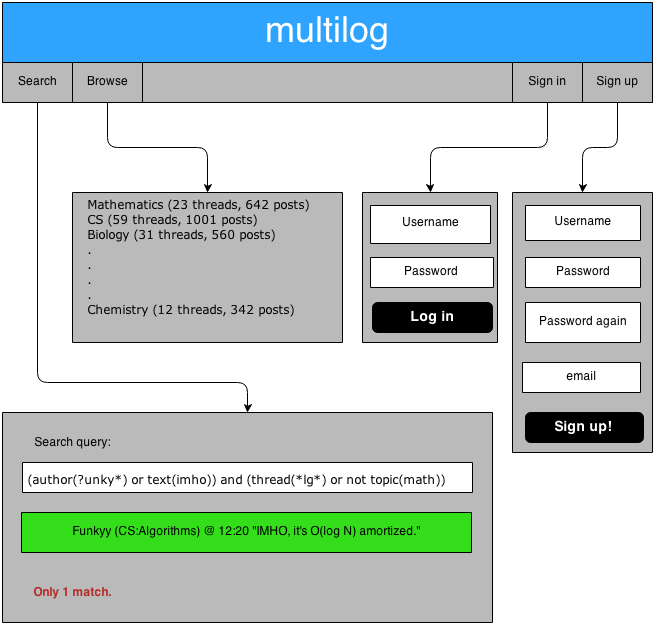
\includegraphics[width=\textwidth, keepaspectratio]{UIMainPage}
\end{figure}

\begin{figure}
  \caption{Profiilinäkymä}
  \centering
  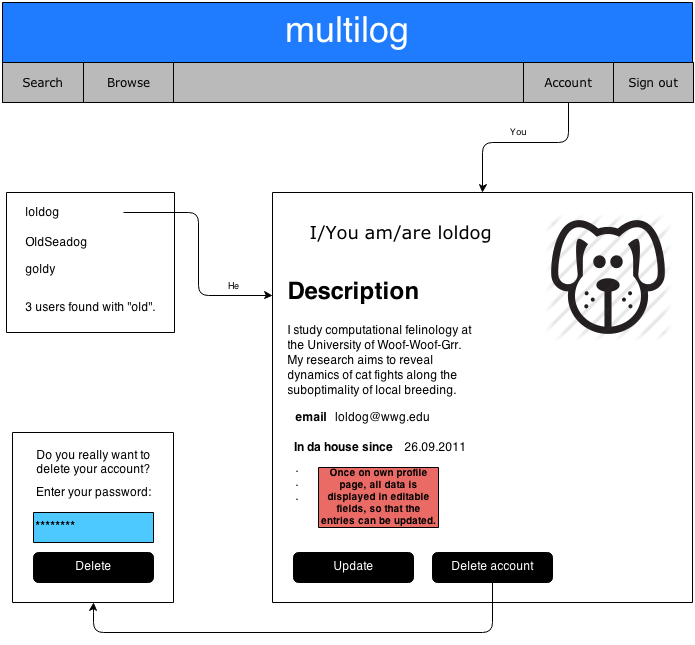
\includegraphics[width=\textwidth, keepaspectratio]{UIAccountView}
\end{figure}
\begin{figure}
  \caption{Säienäkymä}
  \centering
  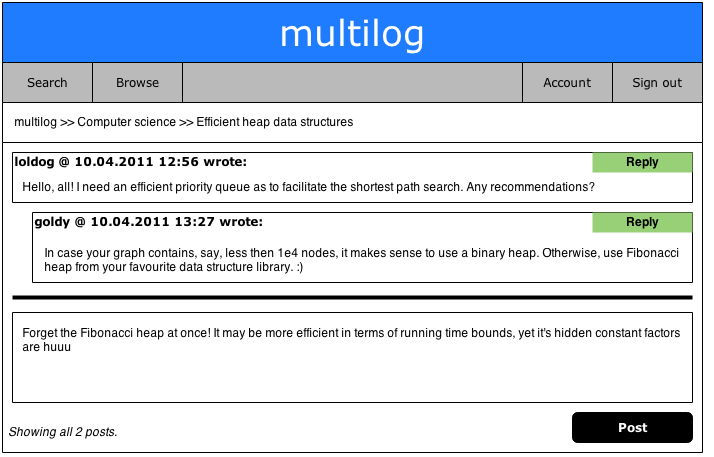
\includegraphics[width=\textwidth, keepaspectratio]{UIThreadView}
\end{figure}
\end{document}